\chapter{Разработка аппаратного описания управляющего устройства}

Все исходные коды аппаратных описаний находятся в директории \emph{/rtl/}.

\section{Описание верхнего уровня}

Описание верхнего уровня находится в файле \emph{/rtl/calsoc\_top.sv}.\\

Управляющее устройство реализовано в виде СнК (Система на кристалле) (\firef{fig:calsoc}) на базе открытого процессорного
ядра \emph{PicoRV32}, основанного на открытой архитектуре RISC-V.

Все периферийные модули подключаются к ядру через шину \emph{Wishbone}. Арбитраж на шине выполняет открытый модуль
\emph{wbxbar}.

\begin{figure}[ht!] 
	\center
	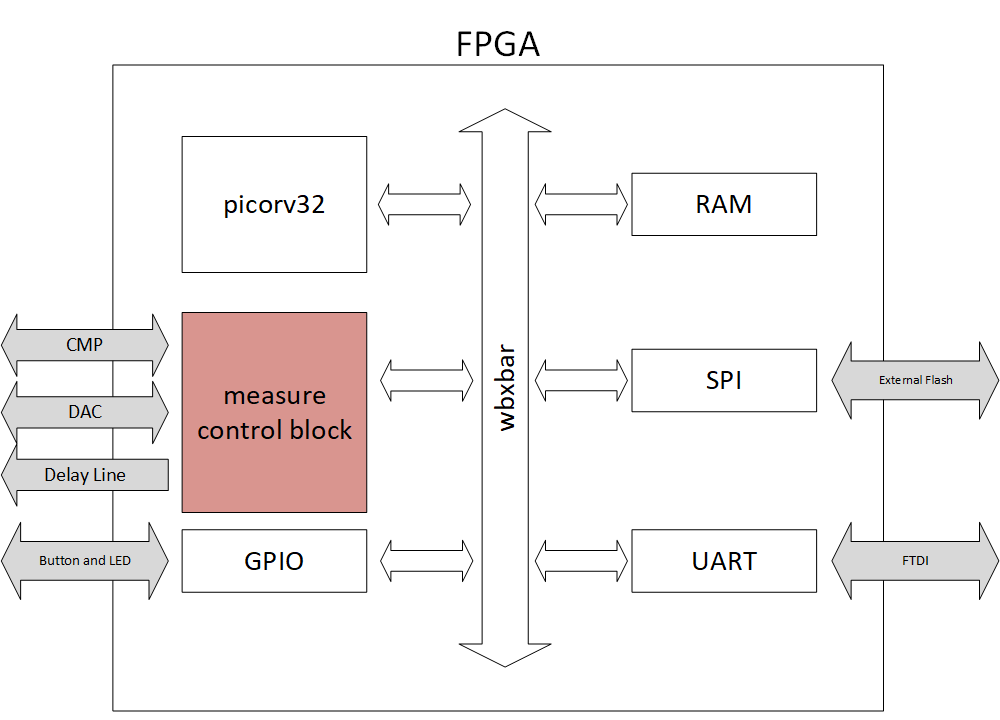
\includegraphics [scale=0.7] {my_folder/images//calsoc}
	\caption{Структурная схема СнК} 
	\label{fig:calsoc}  
\end{figure}

Все периферийные устройства разделяют между собой общее адресное пространство.

\begin{itemize}[label={}]
	\item 0x00000000 -- 0x00FFFFFF -- RAM 
	\item 0x01000000 -- 0x01FFFFFF -- ROM загрузичка
	\item 0x02000000 -- 0x02FFFFFF -- GPIO
	\item 0x03000000 -- 0x03FFFFFF -- UART1
	\item 0x04000000 -- 0x04FFFFFF -- память программы
	\item 0x05000000 -- 0x05FFFFFF -- измерительный модуль
\end{itemize}


\section{Измерительный модуль}

Измерительный модуль выдаёт все необходимые управляющие сигналы для проведения измерений и логически разделён на несколько компонентов:

\begin{itemize}
	\item \emph{stb\_gen} -- модуль, измеряющий частоту сигнала и генерирующий стробы
	\item \emph{ch\_measure\_ctl} -- модуль, непосредственно управляющий измерением одного канала

\end{itemize}


\newpage